
The moment of inertia $I$ of a point mass of mass $m$,
with respect to a given rotation axis is defined as $I = m d^2$
where $d$ is the distance from the point mass to the axis.
This quantity relates the angular velocity $\omega$, 
about the rotation axis,
to the angular momentum $J$, of the point mass, in $J = I \omega$.
This is an analogous relation as the one between the linear momentum $p$
and the linear velocity $v$, $p = m v$. 
For an extended mass distribution in a volume $V$,
a moment of inertia tensor, $I_{ij}$,
relating the angular momentum vector ${\bf J}$ to the rotation vector ${\bf \Omega}$
can be defined as $J_i = I_{ij} \Omega_j$, where the summation convention for repeated
indices is implied.
This tensor is described by a $3 \times 3$ matrix defined by volume integration
over point masses in the volume.
Here we only consider spherically symmetric mass distributions where
the moment tensor is isotopric, $I_{ij} = I \delta_{ij}$,
with scalar coefficient $I$.
\footnote{
$\delta_{ij}$ is the Kronecker delta, i.e. $\delta_{ij}=1$ for
$i=j$ and zero otherwise. }
In simple terms, the moment of inertia is the same for any rotation axis
through the centre of the spherically symmetric body.

The moment of inertia $I$ can be determined from Earth's global gravity
field and the precession rate of the rotation axis determined 
from astronomical data, see Bullen, {\it The Earth's density}, 1975.


The scalar moment of inertia is defined as
a volume integral over point masses,
\begin{mdframed}[backgroundcolor=blue!5]
\begin{equation}
I = \int_V \rho(\vec{r}) d(\vec r)^2 dV. \label{eq:momI}
\end{equation}
\end{mdframed}
where $d(\vec r)$ is the distance from point $\vec{r}$ to the rotation axis.

For a {\it spherically symmetric} body of finite volume, 
it is often expressed in terms of the total mass $M$, the outer radius $R$ 
and a prefactor $f$ as,
\begin{equation}
\boxed{    I = f M R^2}
\label{def_momint_prefact}
\end{equation}

\begin{center}
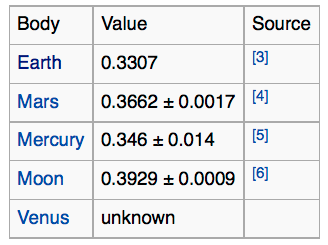
\includegraphics[width=6cm]{images/gravity/moments}\\
{\captionfont Taken from Wikipedia\footnote{\url{https://en.wikipedia.org/wiki/Moment_of_inertia_factor}}}
\end{center}

We have seen that the planetary mass and surface density were used to
constrain models for the interior density distribution.
These models are further constrained by the planets moment of inertia $I$
that can be determined from (satellite) geodetic and astronomical
observations.
For Earth the following values for the total mass and moment of inertia
prefactor have been found,
\begin{eqnarray}
M &=& 5.97 \cdot 10 ^{24}\si{\kilo\gram} \nonumber\\
I &=& 0.3307 M R^2  \si{\kilo\gram\square\metre} \nonumber
\end{eqnarray}
where $R = 6371\si{\kilo\metre}$ is the mean radius.
The observed moment of inertia prefactor $f=0.3307$ is smaller than the 
value $0.4$ for a homogeneous sphere 
(see problem \ref{momint_homogeneous_sphere}), 
%(see \ref{sect_scalarmomint}), 
another indication of mass concentration towards the earth's centre.

\vspace{0.5cm}
\fbox{
\begin{minipage}{0.9\textwidth}
\begin{problem}
 {\small \it
  Derive the following expression for the moment of inertia of a 
  spherically symmetric Earth model with outer radius $R$,
  \begin{equation}
   I = \frac{8 \pi}{3} 
       \int_0^R \rho (r) r^4 dr
  \label{mominert_uniform_sphere}
  \end{equation}
  {\it Hint:} use the symmetry and compute 
  $I = \frac{1}{3} (I_x + I_y + I_z )$,
  where $I_x$ is the moment of inertia with respect to a rotation axis coinciding
  with the $x$-axis.
 }
\end{problem}
\end{minipage}
}

\vspace{0.5cm}
\fbox{
\begin{minipage}{0.9\textwidth}
\begin{problem}
\label{momint_homogeneous_sphere}
{\small \it
  Derive from Eq.~(\ref{mominert_uniform_sphere}) the value of the 
  prefactor $f$ of the moment of inertia for a uniform sphere.
  {\it answer:} $f=2/5$.

In general the moment of inertia prefactor $f$ is an indicator of the
degree of mass concentration towards the centre of a spherically 
symmetric mass distribution. 
Endmembers of mass concentration are 
a) a concentrated central point mass and 
b) all mass concentrated on a spherical surface of zero thickness.

   Verify that the moment of inertia of the point mass endmember 
   equals zero
   and that for the prefactor for a spherical shell of vanishing thickness 
   we have $f=\frac{2}{3}$. 
}
\end{problem}
\end{minipage}
}

\vspace{0.5cm}

Wiechert's two-layer model with a distinct core is constrained 
by the moment of inertia prefactor $f$, the mantle radius $R$ and 
density $\rho_m$
and the total mass $M$ or, equivalently, 
the mean density $\left < \rho \right >$.
Expressions for the core radius $R_c$ and density $\rho_c$   
can be formulated for this model as specified in the following exercise 
(Bullen, 1975).


\vspace{0.5cm}
\fbox{
\begin{minipage}{0.9\textwidth}
\begin{problem}
\label{problem-wiechert-2layermodel}
 {\small \it
  Derive a 2-parameter model for the earth's 1-D radial density 
  distribution $\rho(r)$ consisting of two uniform layers
  (core and mantle) of radius $R_c$ and $R$ respectively and
  with contrasting uniform densities $\rho_c$ and $\rho_m$ for 
  core and mantle respectively.
  Assume $\rho_m$ to be known, leaving $\rho_c$ and $R_c$ as
  unknown parameters that can be determined from the known 
  moment of inertia prefactor $f$ and the average density 
   $\left <\rho \right >$. 

Compute the total mass M

Compute the average density and arrive at:

\begin{equation} 
\left < \rho \right > = \frac{3}{R^3} \int_0^R \rho(r) r^2 dr
\end{equation} 

Use $I=fMR^2$ and the total mass to arrive at:
  \begin{equation} 
    f R^5 \left < \rho \right > = 2 \int_0^R \rho(r) r^4 dr
  \end{equation} 



  Derive the following expressions for $R_c$ and $\rho_c$,
  \begin{equation} 
     \frac{R_c}{R}
       =
     \left (
       \frac{\frac{5}{2}f \frac{\left < \rho \right >}{\rho_m} -1}
            { \frac{\left <\rho \right >}{\rho_m} -1}
    \right )^{1/2}
    ~,~~
     \rho_c = 
        \rho_m 
        \left \{ 1 + 
                 \left ( \frac{R}{R_c} \right )^3 
                 \left ( \frac{\left < \rho \right >}{\rho_m} -1 \right ) 
       \right \}
%%   \rho_c = \rho_m + \left ( \frac{R_c}{R} \right )^{-3}
%%            \left ( \frac{<\rho >}{\rho_m} -1 \right )
  \end{equation} 



 }



\end{problem}
\end{minipage}
}

\vspace{0.5cm}

In Bullen's two-layer model the core radius is assumed to be known
from seismology.
For this model the mantle and core densities can be expressed in the
known parameters in the following problem.


\vspace{0.5cm}
\fbox{
\begin{minipage}{0.9\textwidth}
\begin{problem}
\label{problem-jeffreys-2layermodel}
 {\small \it
  Assume the core radius $R_c$ to be a known parameter in the 
  following.
  Derive a 2-parameter model for the earth's 1-D radial density 
  distribution $\rho(r)$ consisting of two uniform layers
  (core and mantle), with a core and mantle radius $R_c$ and $R$ and
  different uniform densities $\rho_m$ and $\rho_c$ for 
  mantle and core.
  Express the parameters $\rho_m$ and $\rho_c$ in terms of the
  mass and moment of inertia.

  {\it Hint:} compute $M$ first, then $I$, as a function of all other parameters.
  Establish a relationship of the form $(M,I)^T={ A}\cdot (\rho_c,\rho_m)^T$ where
  $A$ is a $2\times2$ matrix.

  {\it Solution:} in matrix-vector format,
  \begin{equation}
  \label{matvec-density-expr-dim}
    \left (
        \begin{array}{c}
               \rho_c \\
               \rho_m \\
        \end{array}
   \right )
   =
   \frac{4\pi}{3\Delta}
    \left (
        \begin{array}{cc}
               \frac{2}{5}(R^5-R_c^5) & -(R^3-R_c^3) \\
              -\frac{2}{5}R_c^5       & R_c^3        \\
        \end{array}
   \right )
    \left (
        \begin{array}{c}
                   M \\
                   I \\
        \end{array}
   \right )
  \end{equation}
  where the determinant 
     $\Delta = \frac{32\pi^2}{45} 
               \left (
                 R_c^3 (R^5 -R_c^5) - R_c^5 (R^3-R_c^3)
              \right ) $.
 }
\end{problem}
\end{minipage}
}

\vspace{0.5cm}





\vspace{0.5cm}
\fbox{
\begin{minipage}{0.9\textwidth}
\begin{problem}
SKIP THIS PROBLEM.
{\small \it
The numerical value of the interim expressions in 
(\ref{matvec-density-expr-dim}) exceeds the magnitude of 
single precision real type variables in computer programs,
that are limitid to approximately $1.7 \cdot 10^{38}$.
A work around for this problem may be to use double precision 
real variables that have a higher maximum magnitude
of about $10^{308}$.

An alternative solution is to switch to using non-dimensional 
parameters, denoted by primes, in the following way:
define 
$R_c^{'} =R_c/R$,
$M_0= 4/3 \cdot \pi R^3 \rho_0 $ and %$M^{'}=1$.
$M= M_0 \cdot M/M_0 = M_0 \cdot M^{'}$,
$\rho_c=\rho_0 \rho_c^{'}$,
$\rho_m=\rho_0 \rho_m^{'}$ and express the moment of inertia 
in the reference density $\rho_0$ and outer radius as,
$I = f M R^2= f 4/3\cdot \pi R^5 \rho_0 $.
With these definitions rewrite (\ref{matvec-density-expr-dim}) 
into the non-dimensional form,
  \begin{equation}
  \label{matvec-density-expr-nondim}
    \left (
        \begin{array}{c}
               \rho_c^{'} \\
               \rho_m^{'} \\
        \end{array}
   \right )
   =
   \frac{16\pi^2}{9\Delta^{'}}
    \left (
        \begin{array}{cc}
               \frac{2}{5}(1-R_c^{'5}) & -(1-R_c^{'3}) \\
              -\frac{2}{5}R_c^{'5}     & R_c^{'3}      \\
        \end{array}
   \right )
    \left (
        \begin{array}{c}
                   M^{'} \\
                   f \\
        \end{array}
   \right )
  \end{equation}
  where the determinant 
     $\Delta^{'} = \frac{32\pi^2}{45} 
               \left (
                 R_c^{'3} (1 -R_c^{'5}) - R_c^{'5} (1-R_c^{'3})
              \right ) $.
 }
\end{problem}
\end{minipage}
}

\vspace{0.5cm}

%%\begin{problem}
%%  Show that the moment of inertia can be split in separate contributions
%%  from the mantle and the core, $I = I_m + I_c$.
%%
%%  Derive expressions for $I_m$ and $I_c$ for the above model with uniform 
%%  mantle and core in terms of the masses of equivalent spheres with
%%  radius $R$ and $R_c$ and densities $\rho_m, \rho_c$ and 
%%  the density contrast
%%  $\Delta \rho = \rho_c - \rho_m$.
%%
%%  Show from these expressions that the moment of inertia prefactor $f$
%%  of the two-layer model is smaller or greater than 0.4 in cases where
%%  $\Delta \rho$ is positive or negative respectively.
%%  \newline
%%  {\it Hint:}
%%  Derive an expression for the prefactor $f$ in terms of $\Delta \rho$.
%%\end{problem}

